\documentclass{article}
\usepackage[margin=2cm]{geometry}
\setlength{\parindent}{0pt}
\usepackage{amsmath}
\usepackage{tikz}
\usepackage{esvect}
\newcommand\myvv[1]{\mkern1.5mu\vec{\mkern-1.5mu#1}}
\usepackage{hyperref}

\title{Simple Ball Collision Calculations}
\author{Peleg Bar Sapir}

\begin{document}
\maketitle
\section{Ball-Ball Collision}
\subsection{Problem}
At a time $t_{0}=0$ two perfectly spherical balls with radii $r_{i}$ and masses $m_{i}$ ($i\in{1,2}$) 

\vspace{1em}
\underline{Illustration}:
\begin{center}
    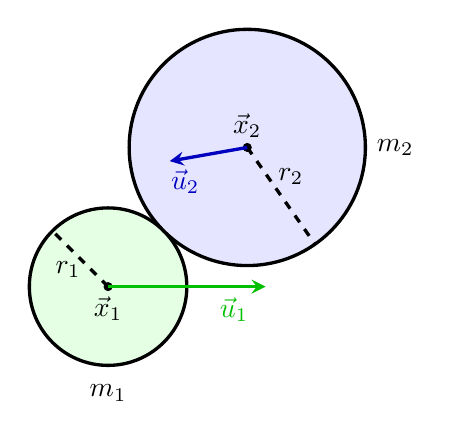
\begin{tikzpicture}
        \tikzset{vector/.style={-stealth, very thick}}
        \pgfmathsetmacro{\angle}{45}
        \pgfmathsetmacro{\ra}{1.0}
        \pgfmathsetmacro{\rb}{1.5}
        \coordinate (x1) at (0,0);
        \coordinate (x2) at ({(\ra+\rb)*cos(\angle)},{(\ra+\rb)*sin(\angle)});
        \draw[very thick, black, fill=green!10] (x1) circle (\ra);
        \draw[very thick, black, fill=blue!10] (x2) circle (\rb);
        \filldraw[black] (x1) circle (0.05) node[below] {$\vec{x}_{1}$};
        \filldraw[black] (x2) circle (0.05) node[above] {$\vec{x}_{2}$};
        \draw[very thick, dashed] (x1) -- (135:\ra) node[pos=0.3, left] {$r_{1}$};
        \draw[very thick, dashed] (x2) -- ++(305:\rb) node[pos=0.3, right] {$r_{2}$};
        \node[below of=x1, yshift=-10pt] {$m_{1}$};
        \node[right of=x2, xshift=25pt] {$m_{2}$};
        \draw[vector, green!75!black] (x1) -- (0:2.0) node[pos=.8, below] {$\vec{u}_{1}$};
        \draw[vector, blue!75!black] (x2) -- ++(190:1.) node[pos=.8, below] {$\vec{u}_{2}$};
    \end{tikzpicture}
\end{center}


\begin{enumerate}
    \item What is the time $t$ of the collision?
    \item What are the positions $\vec{x}_{i}$ of their centers at that time?
    \item What are the velocities $\vec{v}_{i}$ after the collision?
\end{enumerate}

\subsection{Solution}
% \underline{Note}: the solution given here is based on the text in \href{https://www.sjsu.edu/faculty/watkins/collision.htm}{this webpage}.
%
% \vspace{1em}
% Conservation of momentum gives
% \begin{equation}
%     m_{1}\vec{u}_{1} + m_{2}\vec{u}_{2} = m_{1}\vec{v}_{1} + m_{2}\vec{v}_{2},
%     \label{eq:conservation_of_momentum_1}
% \end{equation}
% i.e.
% \begin{equation}
%     m_{1}\left(\vec{u}_{1}-\vec{v}_{1}\right) = -m_{2}\left(\vec{u}_{2}-\vec{v}_{2}\right).
%                     \label{eq:conservation_of_momentum_2}
% \end{equation}
%
% Conservation of (kinetic) energy gives
% \begin{equation}
%     \frac{1}{2}m_{1}u_{1}^{2} + \frac{1}{2}m_{2}u_{2}^{2} = \frac{1}{2}m_{1}v_{1}^{2} + \frac{1}{2}m_{2}v_{2}^{2},
%     \label{eq:conservation_of_energy_1}
% \end{equation}
% which can be further simplified using the dot product (since for any vector $\vec{w}$, $w^{2}=\vec{w}\cdot\vec{w}$) and eliminating the $\frac{1}{2}$ coefficient, leaving us with
% \begin{equation}
%     m_{1}\left( \vec{u}_{1}\cdot\vec{u}_{1} - \vec{v}_{1}\cdot\vec{v}_{1} \right) = -m_{2}\left( \vec{u}_{2}\cdot\vec{u}_{2} - \vec{v}_{2}\cdot\vec{v}_{2} \right),
%     \label{eq:conservation_of_energy_2}
% \end{equation}
% i.e. (utilizing $a^{2}-b^{2}=(a-b)(a+b)$)
% \begin{equation}
%     m_{1}\left( \vec{u}_{1}-\vec{v}_{1} \right)\cdot\left( \vec{u}_{1}+\vec{v}_{1} \right) = m_{2}\left( \vec{u}_{2}-\vec{v}_{2} \right)\cdot\left( \vec{u}_{2}+\vec{v}_{2} \right).
%     \label{eq:conservation_of_energy_3}
% \end{equation}
%
% The change in momentum must happen along the line connecting the centers of the balls. We can easily derive the vector connecting $\vec{x}_{2}$ to $\vec{x}_{1}$:
% \begin{equation}
%     \vec{X} = \vec{x}_{1}-\vec{x}_{2},
%     \label{eq:connect_x1_x2}
% \end{equation}
% and normalize it to
% \begin{equation}
%     \hat{X} = \frac{\vec{x}_{1}-\vec{x}_{2}}{\left\|\vec{x}_{1}-\vec{x}_{2} \right\|} = \frac{\vec{X}}{r_{1}+r_{2}}.
%     \label{eq:unit_connect_x1_x2}
% \end{equation}
%
% The change in momentum is this given by
% \begin{equation}
%     m_{1}\left( \vec{u}_{1}-\vec{v}_{1} \right) = -m_{2}\left( \vec{u}_{2}-\vec{v}_{2} \right) = \alpha\hat{X},
%     \label{eq:change_in_momentum}
% \end{equation}
% where $\alpha\in\left(0, \infty\right)$.
%
% We can use \autoref{eq:change_in_momentum} to express \autoref{eq:conservation_of_energy_3} as
% \begin{equation}
%     \hat{X}\cdot\left(\vec{u}_{1}+\vec{v}_{1}\right) = \hat{X}\cdot\left(\vec{u}_{2}+\vec{v}_{2}\right),
%     \label{eq:label}
% \end{equation}
% and using \autoref{eq:change_in_momentum} we get the following expressions for the velocities $\vec{v}_{i}$:
% \begin{align}
%     \vec{v}_{1} &= \vec{u}_{1} - \frac{\alpha}{m_{1}}\hat{X},\nonumber\\
%     \vec{v}_{2} &= \vec{u}_{2} + \frac{\alpha}{m_{2}}\hat{X}.
%     \label{eq:v_from_u}
% \end{align}
%
% The only thing left to do is to find $\alpha$. Applying \autoref{eq:v_from_u} to \autoref{eq:conservation_of_energy_3} we find that
% \begin{equation}
%     \hat{X}\cdot\left(2\vec{u}_{1}-\frac{\alpha}{m_{1}}\hat{X}\right) = \hat{X}\left(2\vec{u}_{2}+\frac{\alpha}{m_{2}}\hat{X}\right).
%     \label{eq:find_alpha}
% \end{equation}
% and since $\hat{X}$ is a unit vector, i.e. $\hat{X}\cdot\hat{X}=1$, the above reduces to
% \begin{equation}
% 2\hat{X}\cdot\left(\vec{u}_{1}-\vec{u}_{2}\right) = \alpha\left(\frac{1}{m_{1}}+\frac{1}{m_{2}}\right),
%     \label{eq:reduction_1}
% \end{equation}
% and thus
% \begin{equation}
% \alpha = \frac{2\hat{X}\left(\vec{u}_{1}-\vec{u}_{2}\right)}{\frac{1}{m_{1}}+\frac{1}{m_{2}}}.
%     \label{eq:reduction_2}
% \end{equation}
%
% To simplify things further, we can define two more quantities:
% \begin{align}
%     \Delta \vec{u} &= \vec{u}_{1}-\vec{u}_{2},\\
%     \mu &= \frac{1}{\frac{1}{m_{1}}+\frac{1}{m_{2}}},
%     \label{eq:simplifications_1}
% \end{align}
% and then \autoref{eq:reduction_2} simplifies to
% \begin{equation}
%     \alpha = 2\mu\hat{X}\Delta\vec{u}.
%     \label{eq:simplifications_2}
% \end{equation}
\end{document}
